\section{Methodology}\label{sec:method-dataloc}
This section first formalizes the repository-level code localization problem. It then analyzes the intrinsic challenges that motivate the hybrid approach, \tooldataloc, which combines the strengths of large language models with the rigorous logical reasoning of Datalog.

\begin{landscape}
\begin{figure}[t]
	\centering
	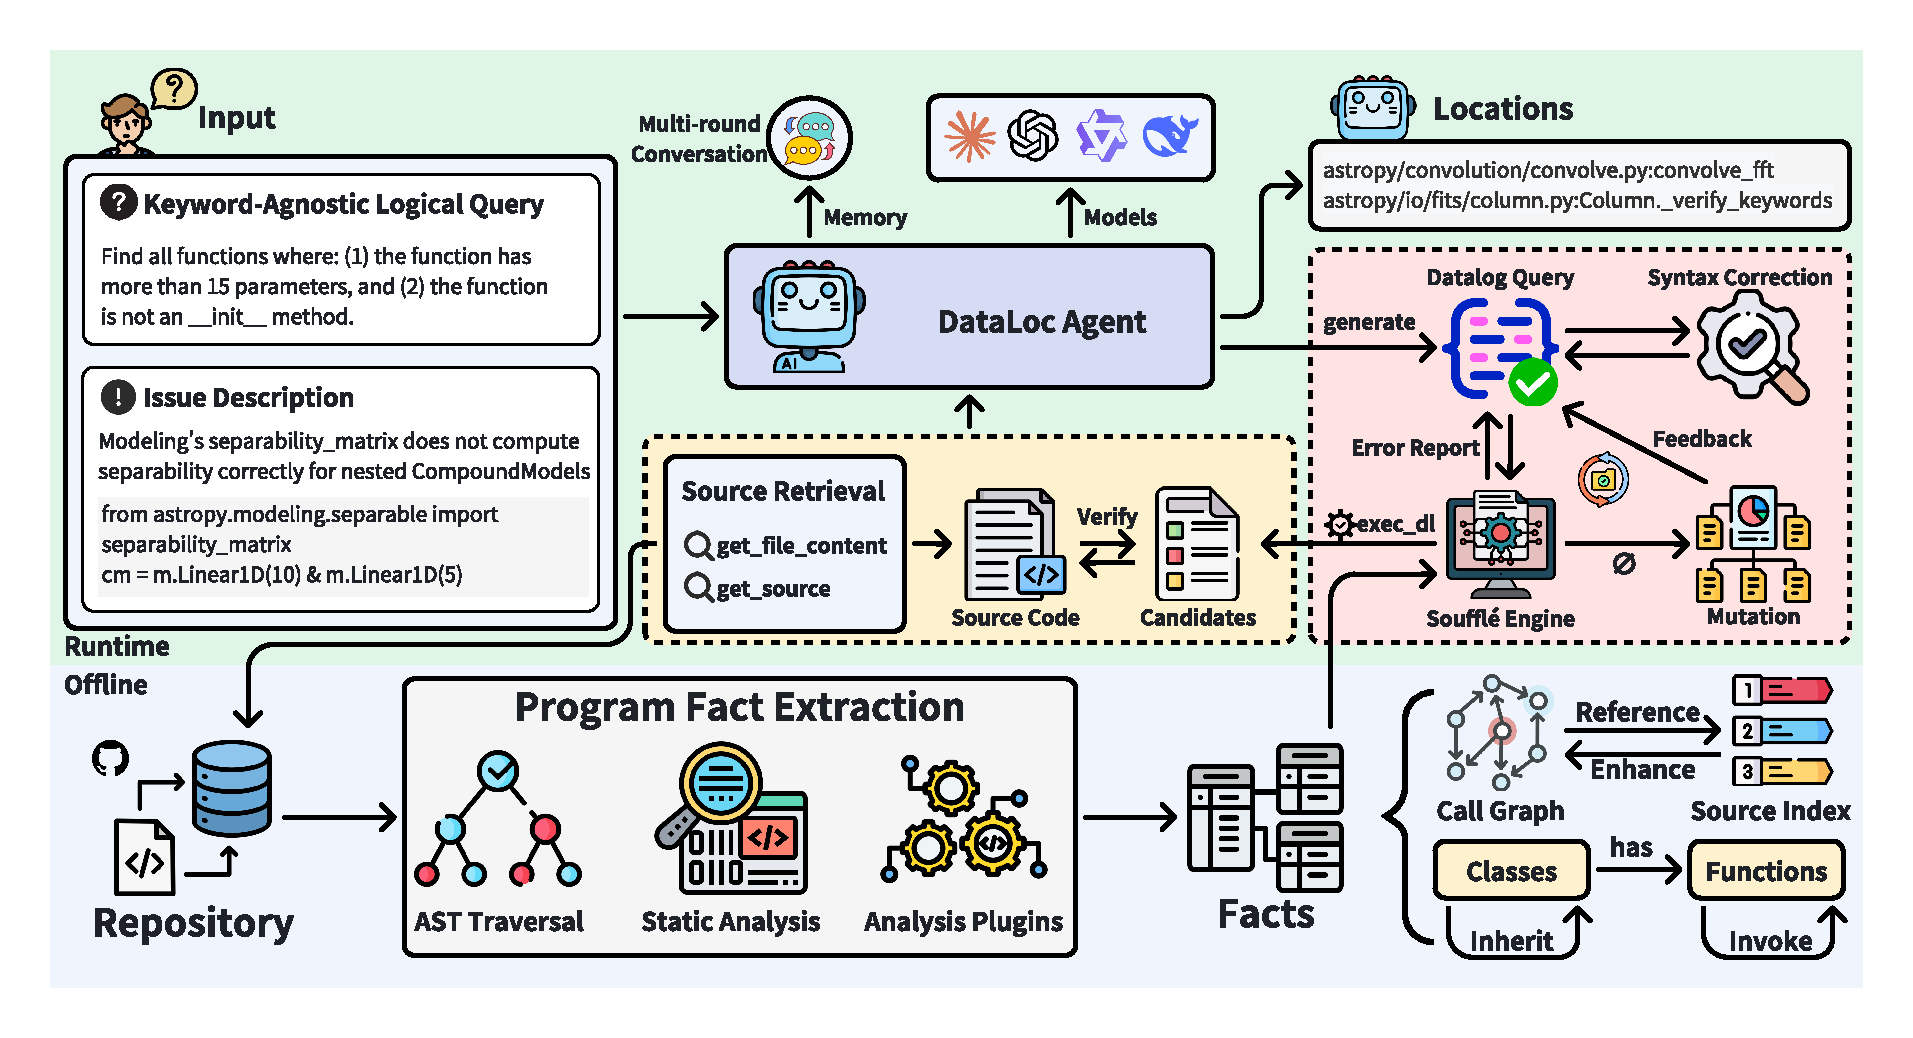
\includegraphics[width=\linewidth]{Figures/Chapter5/architecture.pdf}
	\caption{Overview of the \tooldataloc framework.}
	\label{fig:arch-dataloc}
\end{figure}
\end{landscape}


Given a natural language query $q$ (e.g., a bug report or feature request) and a target codebase $\mathcal{C}$, the goal of \textbf{repository-level code localization} is to identify a list of relevant code locations $\mathcal{L}=\{l_1, l_2, \dots, l_k\}$. Effective localization bridges the gap between informal natural language and the rigid execution logic of software. Three primary challenges are identified:

\begin{itemize}[leftmargin=*]
    \item \textbf{Challenge 1: Semantic and Lexical Disconnect.} There exists a non-trivial gap between the informal vocabulary of $q$ and the formal identifiers in $\mathcal{C}$. This disconnect is categorized into three progressive layers: (1) \textit{Keyword Absence}, where a query lacks any direct textual anchors present in the code; (2) \textit{Latent Semantic Mapping}, where high-level task descriptions (e.g., \texttt{login failure}) lack direct textual overlap with low-level implementation entities (e.g., \texttt{AuthManager} or \texttt{ValidateToken}); (3) \textit{Lexical Divergence}, where developers use synonyms or abbreviations (e.g., \texttt{fqn} for \texttt{fullyQualifiedName}) that elude exact match search.

    \item \textbf{Challenge 2: Non-local Structural Dependencies.} Relevant code is often not directly mentioned in queries but connected through dependencies or calls. A single feature may be implemented across multiple files. For example, identifying \textit{password validation} logic may require traversing complex call chains and data flows scattered across authentication modules and database layers. Existing pipeline-based tools rely on local directory traversal and fail to capture these deep, cross-file relational dependencies.

    \item \textbf{Challenge 3: Complex Logical Pattern Constraints.} Questions may contain logical pattern requirements that candidate code must satisfy. Certain localization tasks are defined by structural patterns rather than keywords. For example, \textit{identifying the conditional statement that raises three distinct error types in different branches} requires satisfying specific logical constraints defined by the language's syntax and semantics. Such patterns are difficult to locate by retrieving class or function information alone; they require repository-level structural understanding and reasoning.
\end{itemize}

To address these challenges, this study proposes \tooldataloc, a synergy between LLMs and Datalog. The underlying intuition is that LLMs excel at resolving \textit{Challenge 1} by translating vague natural language intents into structured requirements, while Datalog provides the relational and reasoning power to solve \textit{Challenge 2} and \textit{Challenge 3} by evaluating relational constraints over the extracted facts.
In the proposed framework, the codebase $\mathcal{C}$ is represented as a set of pre-extracted program facts $\mathcal{F}$, where $\mathcal{F}$ captures both the source entities and the structural relations, such as function-call information, class membership, and declared inheritance relationships. Each location $l_i \in \mathcal{L}$ corresponds to a specific level of granularity, such as a file, module, or function, that is essential for resolving the query $q$. \fref{fig:arch-dataloc} illustrates the overview of the framework of \tooldataloc. The framework operates in two stages. First, an offline program fact extraction stage analyzes the codebase to build a structured knowledge base. Second, an automated agent execution stage leverages these extracted facts to perform code localization by synthesizing high-quality Datalog queries.

\subsection{Program Facts Extraction}\label{sec:fact-extraction-dataloc}
This subsection describes the details of extracting program facts from a given repository.
Program facts are extracted through a modular pipeline that separates source discovery, structural parsing, and fact emission, shown as the offline \textit{Program Fact Extraction} stage in \fref{fig:arch-dataloc}. First, the extraction pipeline enumerates source files under the repository root using the configured file-selection rules. A language-specific frontend then analyzes the files using the most suitable intermediate representation. For Python, the frontend parses source code into an abstract syntax tree and emits facts during traversal. The frontend produces Datalog facts annotated with precise source locations and stable identifiers, enabling traceability and incremental updates.

These frontends emit facts describing program entities (files, modules, functions, classes, variables) and relations (containment, inheritance, import/use, call, and reference edges), together with optional control flow and data flow information when available. This representation directly addresses \textit{Challenge 2} by making cross-file interactions explicit and queryable~\cite{wu2021diffbase}. Instead of relying on local directory traversal, localization can now operate over global dependency graphs, enabling the identification of code relevant to a feature even when it is scattered across multiple modules and layers.

The extracted facts also enable expressive logical pattern matching, which helps solve \textit{Challenge 3}. Structural requirements, such as specific exception patterns or multi-step call sequences, can be formulated as Datalog queries over extracted facts. This allows localization tasks defined by program structure rather than surface keywords to be handled systematically, without requiring the LLM to reason over raw source code.

\subsubsection{Relational Schema and Extraction Semantics}\label{sec:facts-schema-dataloc}
Following the relational representation introduced in \sref{sec:background-program-facts-datalog}, the Python fact interface used in this study comprises 17 relations. Table~\ref{tab:dataloc-fact-schema} lists these relations with their original argument names and order. Each relation contains a finite set of tuples extracted from the analyzed repository snapshot, with argument types specified below. Line numbers, column positions, span bounds, counts, and parameter indices have type \texttt{number}; all other arguments have type \texttt{symbol}, including Boolean flags represented as \texttt{True} and \texttt{False}.

\begin{table}[htbp]
\centering
\caption{Python program-fact relations and their arguments.}
\label{tab:dataloc-fact-schema}
\begingroup
\setstretch{1}
\fontsize{9.5}{11}\selectfont
\renewcommand{\arraystretch}{1.05}
\setlength{\tabcolsep}{6pt}
\begin{tabularx}{\linewidth}{@{}l>{\raggedright\arraybackslash}X@{}}
\toprule
Relation & Arguments in declaration order \\
\midrule
\texttt{source\_file} & \mbox{\texttt{file\_path}}, \mbox{\texttt{content\_hash}}, \mbox{\texttt{total\_lines}} \\
\texttt{source\_line} & \mbox{\texttt{file\_path}}, \mbox{\texttt{line\_number}}, \mbox{\texttt{content}} \\
\texttt{ast\_node} & \mbox{\texttt{file\_path}}, \mbox{\texttt{line}}, \mbox{\texttt{column}}, \mbox{\texttt{node\_type}}, \mbox{\texttt{parent\_line}}, \mbox{\texttt{parent\_column}} \\
\texttt{class\_definition} & \mbox{\texttt{file\_path}}, \mbox{\texttt{class\_name}}, \mbox{\texttt{start\_line}}, \mbox{\texttt{end\_line}}, \mbox{\texttt{base\_class}} \\
\texttt{class\_nesting} & \mbox{\texttt{file\_path}}, \mbox{\texttt{nested\_class}}, \mbox{\texttt{parent\_class}}, \mbox{\texttt{line}} \\
\texttt{class\_method} & \mbox{\texttt{file\_path}}, \mbox{\texttt{class\_name}}, \mbox{\texttt{method\_name}}, \mbox{\texttt{line}}, \mbox{\texttt{is\_static}}, \mbox{\texttt{is\_class\_method}} \\
\texttt{class\_attribute} & \mbox{\texttt{file\_path}}, \mbox{\texttt{class\_name}}, \mbox{\texttt{attribute\_name}}, \mbox{\texttt{line}}, \mbox{\texttt{attribute\_type}} \\
\texttt{function\_definition} & \mbox{\texttt{file\_path}}, \mbox{\texttt{function\_name}}, \mbox{\texttt{start\_line}}, \mbox{\texttt{end\_line}}, \mbox{\texttt{param\_count}}, \mbox{\texttt{is\_async}}, \mbox{\texttt{containing\_class}} \\
\texttt{function\_parameter} & \mbox{\texttt{file\_path}}, \mbox{\texttt{function\_name}}, \mbox{\texttt{function\_line}}, \mbox{\texttt{param\_name}}, \mbox{\texttt{param\_type}}, \mbox{\texttt{default\_value}}, \mbox{\texttt{param\_index}} \\
\texttt{function\_decorator} & \mbox{\texttt{file\_path}}, \mbox{\texttt{function\_name}}, \mbox{\texttt{function\_line}}, \mbox{\texttt{decorator\_name}} \\
\texttt{function\_call} & \mbox{\texttt{file\_path}}, \mbox{\texttt{calling\_function}}, \mbox{\texttt{line}}, \mbox{\texttt{called\_function}}, \mbox{\texttt{arg\_count}}, \mbox{\texttt{call\_type}} \\
\texttt{type\_annotation} & \mbox{\texttt{file\_path}}, \mbox{\texttt{entity\_name}}, \mbox{\texttt{line}}, \mbox{\texttt{type\_expression}}, \mbox{\texttt{annotation\_type}} \\
\texttt{variable\_definition} & \mbox{\texttt{file\_path}}, \mbox{\texttt{variable\_name}}, \mbox{\texttt{line}}, \mbox{\texttt{variable\_type}}, \mbox{\texttt{initial\_value}}, \mbox{\texttt{scope\_name}} \\
\texttt{import\_statement} & \mbox{\texttt{file\_path}}, \mbox{\texttt{line}}, \mbox{\texttt{imported\_name}}, \mbox{\texttt{local\_alias}}, \mbox{\texttt{import\_type}} \\
\texttt{control\_structure} & \mbox{\texttt{file\_path}}, \mbox{\texttt{structure\_type}}, \mbox{\texttt{start\_line}}, \mbox{\texttt{end\_line}}, \mbox{\texttt{condition}} \\
\texttt{exception\_handling} & \mbox{\texttt{file\_path}}, \mbox{\texttt{line}}, \mbox{\texttt{exception\_types}}, \mbox{\texttt{handler\_description}} \\
\texttt{docstring} & \mbox{\texttt{file\_path}}, \mbox{\texttt{entity\_name}}, \mbox{\texttt{line}}, \mbox{\texttt{content}}, \mbox{\texttt{docstring\_type}} \\
\bottomrule
\end{tabularx}
\endgroup
\end{table}

Paths are relative to the repository root, and source spans include both boundary lines in the analyzed snapshot. Method names are class-qualified, as in \texttt{TimeSeries.\_\_init\_\_}. A \texttt{control\_structure} fact records the construct kind, full syntax-tree span, and normalized condition; an \texttt{if} span therefore includes its alternative branches. The \texttt{exception\_handling} relation describes exception-handling constructs, not explicit \texttt{raise} statements.

The facts provide a syntactic representation rather than complete control-flow or data-flow graphs. Calls are recorded without resolving dynamic targets, and condition summaries may omit parts of compound expressions. Constraints not preserved by this representation, such as whether two raises occur in different branches, require source verification, as illustrated in \sref{sec:end-to-end-dataloc}.


\subsection{Agentic Workflow}
This section elaborates on the agent-based workflow for automated repository-level code localization, which builds upon the program facts constructed offline.

The end-to-end agent is designed to accept natural language queries and return precise code locations. Unlike approaches that provide a fixed top-$n$ list of candidates, the system outputs a dynamic set of potential locations to maximize precision. To mitigate hallucinations and enhance abstention ability, the framework decouples reasoning from generation. A deterministic engine handles inference while the LLM acts as a coordinator for query analysis and result calibration. The agent is equipped with three basic tools: \texttt{exec\_dl} for executing Datalog programs, and \texttt{get\_file\_contents} along with \texttt{get\_sources} for retrieving source code and specific line ranges.

\subsubsection{Query Analysis and Information Resolution}
The workflow begins with a preliminary analysis of the query to extract the core technical concepts and structural elements, performed by the \textit{DataLoc Agent} in \fref{fig:arch-dataloc}. By identifying program entities such as file paths, module names, and structure descriptions, the agent establishes an internal context. This preparatory step provides the necessary predicates and constraints for the subsequent synthesis of Datalog programs.

\subsubsection{Synthesize-Check-Refine Loop}
As shown in the red panel in \fref{fig:arch-dataloc}, before execution, \tooldataloc follows a \textit{synthesize-check-refine} loop to mitigate the impact of hallucinations and improve the executability of LLM-generated Datalog programs. It mainly contains two critical, feedback-driven phases (details in \sref{sec:method:val-dataloc} and \sref{sec:method:int-dataloc}): (1) \textit{Syntax correction}. Each synthesized program undergoes parser-gated validation to ensure syntactic well-formedness. The workflow adopts a \emph{best-effort repair, then fallback} strategy: unambiguous cases are handled via conservative rule-based fixes, revalidated with \souffle's parser, and all other cases return error feedback to the LLM. (2) \textit{Intermediate-rule diagnosis}. The diagnostic mechanism instruments the program to track row counts of intermediate relations, thereby identifying rules that produce empty results. Controlled mutation probes then classify such emptiness as fragile, stable, or inconclusive, giving the model targeted evidence for refinement. Validated programs are then executed through the \texttt{exec\_dl} tool to generate a list of candidates. Excessive locations are treated as failures, triggering refinement with stricter constraints to reduce noise and improve precision.

\subsubsection{Context Retrieval and Final Verification}
As depicted in the yellow panel in \fref{fig:arch-dataloc}, once a set of potential code locations has been determined, the agent retrieves the relevant code snippets using \texttt{get\_sources} or \texttt{get\_file\_contents} and conducts a verification against the original query. These verified locations are then returned in a standardized format (e.g., \texttt{FILE\_PATH:CLASS.METHOD}). Although the agent may undergo multiple internal reasoning iterations, the user experience is streamlined into a single step: submitting a query and receiving a list of locations. This fully automated closed-loop design ensures both usability and seamless integration into production development environments.



\subsection{Repairing LLM-Generated Datalog}
\label{sec:method:val-dataloc}
LLM-generated Datalog programs (the dialect used by \souffle) often contain syntactic and semantic errors, especially when the model is not fine-tuned for Datalog programming.

As shown in the red panel in \fref{fig:arch-dataloc}, before executing an LLM-generated Datalog program, the framework enforces a \emph{parser-gated validation} workflow to ensure that only syntactically well-formed
programs reach later stages of the pipeline. This design is motivated by the observation that some
failures are caused by superficial syntactic issues that can be repaired mechanically, whereas more
complex parse failures often require global restructuring that is better handled by the LLM. The
workflow therefore follows a \emph{repair-or-feedback} strategy: the workflow applies conservative rule-based fixes when the repair is unambiguous, re-checks the program using \souffle's parser, and otherwise returns error feedback to the LLM.


The workflow invokes a lightweight parser helper (based on \souffle's parsing frontend) to validate the
generated program. If parsing fails, the workflow first attempts a small set of mechanical rewrite rules
targeting high-frequency issues. For example, LLMs frequently introduce naming collisions by using
reserved or special identifiers as variable names.
One common case is using \texttt{count} as a variable name while it is a reserved keyword in
\souffle.
Such cases can be fixed locally via deterministic renaming.

However, not all parser errors admit a reliable deterministic repair.
In these cases, the workflow does not attempt speculative transformations. Instead, the workflow returns the raw parser diagnostics (optionally augmented with concise hints) to the LLM, allowing the model to revise the program directly.

Any program that fails parser validation is rejected and never proceeds to later stages. Once a
program passes syntactic validation (either initially or after rule-based repair), the workflow applies semantic correctness checks that encode \souffle-specific usage rules and common domain
conventions. These checks detect syntactically valid but semantically incorrect programs arising
from common misconceptions in LLM-generated Datalog code. Only programs that satisfy both syntactic
and semantic validation proceed to execution.

A representative example is the use of string containment constraints. \souffle provides a constraint function
\texttt{contains(sub:symbol,full:symbol)}, which is defined such that the second argument must
contain the first (i.e., full includes sub). However, LLMs are observed to frequently invert this
positional relationship by producing atoms like \texttt{contains(content,``keyword'')} instead of
the correct \texttt{contains(``keyword'',content)}.
Since such inversions conform to both the syntax and type specifications, they often lead to silent
failures or empty results that are difficult for LLMs to self-correct, even after multiple rounds
of feedback.

Prompt techniques such as few-shot learning cannot effectively eliminate this kind of error.
Therefore, a library of semantic rules is constructed to check the correct usage of built-in
predicates with non-commutative argument semantics and other similar constraints.
These repairs are applied only when the transformation is high-confidence and semantics-preserving.
When uncertain, the checker records the issue for subsequent feedback to the LLM rather than
applying a blind fix, thereby guiding the refinement in subsequent iterations.
The contribution of this mechanism is evaluated through an ablation study in~\sref{sec:ablation-dataloc}, demonstrating its effectiveness in improving synthesis quality.

\subsection{Diagnosing Intermediate Rules via Conservative Mutation Analysis}
\label{sec:method:int-dataloc}

An intermediate-rule diagnostic mechanism is introduced for LLM-generated Datalog programs, corresponding to \textit{Mutation} in the red panel of \fref{fig:arch-dataloc}. As
illustrated in \fref{fig:mutate-dataloc}, rather than evaluating a program solely by its final output,
\tooldataloc instruments intermediate derived relations, records their cardinalities, and applies
diagnostic mutations to relations that derive zero tuples. Since an empty relation may represent
either a legitimate result or an overly restrictive rule, these mutations serve only as diagnostic
probes. Their outputs are used to localize the source of failure and are never returned as part of
the final answer.

\paragraph{Mutation catalog.}
For a zero-cardinality relation~$R$, the diagnostic mechanism mutates only rules that define~$R$. The
catalog is prioritized and capped for cost control; each mutation preserves
the rule head and changes only the body.
\begin{itemize}[leftmargin=*]
\item \textsc{M1. Contains-Literal}: replace each body string
literal \texttt{"s"} with a fresh variable~$V_i$ and append
\texttt{contains("s", $V_i$)}, relaxing exact equality to substring matching.
\item \textsc{M2. Drop-Single-Atom}: remove one selected body atom at
a time while retaining the rest. This general ablation is applied only when a
rule has at least two body atoms and is bounded by a small variant cap.
\item \textsc{M3. Match-Literal}: replace each body string literal
with~$V_i$ and append \texttt{match("s.*", $V_i$)}, testing whether the
literal is a prefix of the actual fact value.
\item \textsc{M4. Drop-Contains}: remove one
\texttt{contains(\ldots)} atom at a time, isolating overly strict string
filters.
\item \textsc{M5. Drop-Single-Negation}: remove one negated atom
(\texttt{!pred(\ldots)}) at a time, probing whether an exclusion constraint is
too strong.
\end{itemize}
M1 and M3 apply only when quoted string literals occur in the rule body; M2, M4, and M5
apply only when their target atom exists and the remaining body still contains
at least one atom.

\paragraph{Feedback construction.}
After applicable probes run, \tooldataloc classifies each zero-cardinality relation as:
\emph{fragile-empty} if any successful mutation yields rows; \emph{stable-empty}
if at least one mutation succeeds and all successful mutations remain empty; and
\emph{inconclusive} if no mutation applies or all probes fail. Feedback reports
the relation name, original zero cardinality, mutation identity, relaxed or removed
constraint, rewritten rule, resulting cardinality, and optionally a small sample of surfaced
tuples.
This gives the LLM evidence for revision without silently weakening the user's intended query
semantics.

\begin{landscape}
\begin{figure}[t]
	\centering
	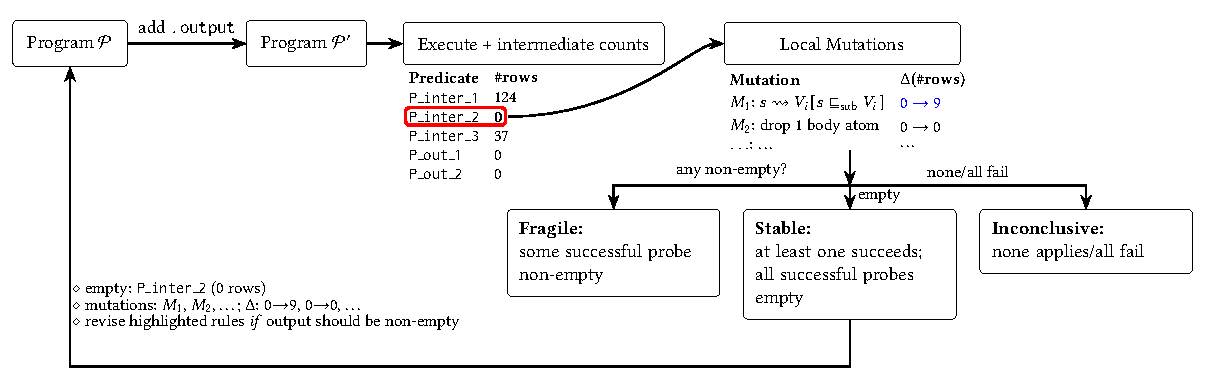
\includegraphics[width=\linewidth]{Figures/Chapter5/mutate.pdf}
	\caption{Intermediate-rule mutation and feedback.}
	\label{fig:mutate-dataloc}
\end{figure}	
\end{landscape}

\subsection{End-to-End Localization Example}\label{sec:end-to-end-dataloc}
\begingroup
\tcbset{datalocstep/.style={
    colback=gray!2, colframe=cyan!40!black, boxrule=0.5pt,
    boxed title style={colback=cyan!6, colframe=cyan!40!black},
    left=2mm, right=2mm, top=3mm, bottom=1.5mm,
    before skip=8pt, after skip=8pt}}
\setminted{fontsize=\footnotesize,baselinestretch=1,breaklines=true,breakautoindent=true}
\setminted[prolog]{xleftmargin=1.5em,numbersep=5pt}
Using Astropy commit \mbox{\texttt{d16bfe05a744909de4b27f5875fe0d4ed41ce607}}, this example traces a recorded localization interaction through the corresponding source code and extracted program facts.

\paragraph*{Original user query.}
The user submits the following localization request:
\begin{quote}
Find all classes where: (1) the \texttt{\_\_init\_\_} method contains an if statement that checks whether a parameter is None, (2) one branch of this if statement raises TypeError and the other branch raises ValueError
\end{quote}

\paragraph*{Relevant facts extracted from the codebase.}
\fref{fig:dataloc-extracted-facts}\subref{fig:dataloc-facts-timeseries} and \subref{fig:dataloc-facts-wcs} show relevant program facts for \texttt{TimeSeries} and \texttt{WCS}, respectively, following the schema in Table~\ref{tab:dataloc-fact-schema} and its accompanying description. These facts record the line ranges of \texttt{\_\_init\_\_} methods and conditionals, together with source lines containing explicit \texttt{raise} statements. 

\begin{landscape}
\begin{figure}[p]
\centering
\begin{subfigure}{\linewidth}
\begin{stepbox}[datalocstep]{Extracted facts: TimeSeries}
\begin{minted}[linenos=false,xleftmargin=0pt]{prolog}
function_definition("astropy/timeseries/sampled.py", "TimeSeries.__init__", 61, 135, 7, False, "TimeSeries").
control_structure("astropy/timeseries/sampled.py", "if_statement", 107, 130, "time_start IsNot None").
source_line("astropy/timeseries/sampled.py", 113, "raise TypeError(\\"'time' is scalar, so 'time_delta' is required\\")").
source_line("astropy/timeseries/sampled.py", 125, "raise ValueError(\\"Length of 'time' ({}) should match \\"").
\end{minted}
\end{stepbox}
\caption{Extracted facts for \texttt{TimeSeries}.}
\label{fig:dataloc-facts-timeseries}
\end{subfigure}
\par\medskip
\begin{subfigure}{\linewidth}
\begin{stepbox}[datalocstep]{Extracted facts: WCS}
\begin{minted}[linenos=false,xleftmargin=0pt]{prolog}
function_definition("astropy/wcs/wcs.py", "WCS.__init__", 380, 546, 12, False, "WCS").
control_structure("astropy/wcs/wcs.py", "if_statement", 391, 527, "header Is None").
source_line("astropy/wcs/wcs.py", 429, "raise TypeError(").
source_line("astropy/wcs/wcs.py", 413, "raise ValueError(").
\end{minted}
\end{stepbox}
\caption{Extracted facts for \texttt{WCS}.}
\label{fig:dataloc-facts-wcs}
\end{subfigure}
\par\medskip
\caption{Relevant program facts from the Astropy repository.}
\label{fig:dataloc-extracted-facts}
\end{figure}
\end{landscape}

\paragraph*{Initially generated Datalog query.}
\fref{fig:dataloc-query-repair}\subref{fig:dataloc-query-initial} shows the initial query generated by the agent. \texttt{InitFunc} targets \texttt{\_\_init\_\_} methods, and \texttt{IfNone} targets enclosed conditionals that test for \texttt{None}. The variable pairs \texttt{f\_start}/\texttt{f\_end} and \texttt{if\_start}/\texttt{if\_end} denote their inclusive line bounds. Argument types are specified in \sref{sec:fact-extraction-dataloc}; \texttt{\_} denotes an anonymous variable.

\paragraph*{Checking, repair, and refinement.}
Exact matching against \texttt{\_\_init\_\_} yields no \texttt{InitFunc} tuples because method names are class-qualified. The empty result triggers a Contains-Literal diagnostic mutation (\sref{sec:method:int-dataloc}), which replaces exact matching of \texttt{\_\_init\_\_} with substring matching. The mutated query produces a nonempty result, yielding \emph{fragile-empty} feedback that identifies the name constraint as a possible cause. Guided by this feedback, the agent inspects the recorded method names and revises the query to match the substring \texttt{.\_\_init\_\_}.

The next candidate query introduces \texttt{RaiseT} and \texttt{RaiseV} for lines containing \texttt{TypeError} and \texttt{ValueError} raises, and \texttt{HasBoth} for conditional spans containing both. It retrieves \texttt{TimeSeries} and \texttt{WCS}. However, finding both exception types within the same conditional span does not establish that they occur in different branches.

\fref{fig:dataloc-query-repair}\subref{fig:dataloc-query-repaired} presents the final query after further agent revisions. Here, \texttt{ST} denotes the recorded control-structure type, \texttt{c} the source-line context, and \texttt{l1} and \texttt{l2} the line numbers of the matched \texttt{TypeError} and \texttt{ValueError} raises, respectively. Compared with the preceding candidate query, it accepts either \texttt{if\_statement} or \texttt{unknown}, requires only the conditional's starting line to fall within the \texttt{\_\_init\_\_} method, and changes the lower-bound checks on raise locations from \texttt{>} to \texttt{>=}. These changes relax the candidate-selection constraints but return the same two candidates. Source verification is therefore still required to determine whether the raises occur in different branches.

Both panels retain the submitted \texttt{contains} argument order, corrected to Souffl\'e's substring-first convention by semantic validation before execution (\sref{sec:method:val-dataloc}). The figure omits only the shared fact-input include directive.

\begin{landscape}
\begin{figure}[p]
\tcbset{datalocstep/.append style={before skip=0pt,after skip=0pt,top=1mm,bottom=1mm}}
\setstretch{1}
\captionsetup{font=small,skip=3pt}
\centering
\begin{subfigure}[t]{\linewidth}
\vspace{0pt}
\centering
\begin{stepbox}[datalocstep]{Initially generated query}
\begin{minted}[linenos=true,fontsize=\fontsize{9}{10}\selectfont,baselinestretch=0.9]{prolog}
.decl InitFunc(file_path: symbol, class_name: symbol, f_start: number, f_end: number)
InitFunc(file_path, containing_class, f_start, f_end) :-
    function_definition(file_path, "__init__", f_start, f_end, _, _, containing_class),
    containing_class != "".
.decl IfNone(file_path: symbol, class_name: symbol, if_start: number, if_end: number, condition: symbol)
IfNone(file_path, class_name, if_start, if_end, condition) :-
    InitFunc(file_path, class_name, f_start, f_end),
    control_structure(file_path, "if_statement", if_start, if_end, condition),
    contains(condition, "None"),
    if_start >= f_start, if_end <= f_end.
.output IfNone
.output InitFunc
\end{minted}
\end{stepbox}
\caption{Initial query for \texttt{\_\_init\_\_} methods and enclosed conditionals.}
\label{fig:dataloc-query-initial}
\end{subfigure}
\par
\begin{subfigure}[t]{\linewidth}
\vspace{0pt}
\centering
\begin{stepbox}[datalocstep]{Final query submitted by the agent}
\begin{minted}[linenos=true,fontsize=\fontsize{9}{10}\selectfont,baselinestretch=0.9,highlightlines={3,4,8,9,10,11,12,13,14,15,16,17,18,19,20},highlightcolor=cyan!8]{prolog}
.decl InitFunc(file_path: symbol, class_name: symbol, f_start: number, f_end: number)
InitFunc(file_path, containing_class, f_start, f_end) :-
    function_definition(file_path, function_name, f_start, f_end, _, _, containing_class),
    containing_class != "", contains(function_name, ".__init__").
.decl IfNone(file_path: symbol, class_name: symbol, if_start: number, if_end: number, condition: symbol)
IfNone(file_path, class_name, if_start, if_end, condition) :-
    InitFunc(file_path, class_name, f_start, f_end),
    control_structure(file_path, ST, if_start, if_end, condition),
    (ST = "if_statement" ; ST = "unknown"),
    contains(condition, "None"), if_start >= f_start, if_start <= f_end.
.decl RaiseT(file_path: symbol, line: number)
RaiseT(file_path, line) :- source_line(file_path, line, c), contains(c, "raise TypeError").
.decl RaiseV(file_path: symbol, line: number)
RaiseV(file_path, line) :- source_line(file_path, line, c), contains(c, "raise ValueError").
.decl HasBoth(file_path: symbol, class_name: symbol, if_start: number, if_end: number, condition: symbol)
HasBoth(file_path, class_name, if_start, if_end, condition) :-
    IfNone(file_path, class_name, if_start, if_end, condition),
    RaiseT(file_path, l1), l1 >= if_start, l1 <= if_end,
    RaiseV(file_path, l2), l2 >= if_start, l2 <= if_end.
.output HasBoth
\end{minted}
\end{stepbox}
\caption{Complete final query, before semantic validation.}
\label{fig:dataloc-query-repaired}
\end{subfigure}
\caption{Initial and complete final queries from the Astropy interaction, with original identifiers and constraints.}
\label{fig:dataloc-query-repair}
\end{figure}
\end{landscape}

\paragraph*{Localization result.}
After semantic validation, the final query returns the following two candidates:
\begin{center}
\footnotesize
\setstretch{1.1}
\setlength{\tabcolsep}{4pt}
\begin{tabular}{@{}lllll@{}}
\toprule
Repository-relative path & Class & Start & End & Condition \\
\midrule
\texttt{astropy/timeseries/sampled.py} & \texttt{TimeSeries} & 107 & 130 & \texttt{time\_start IsNot None} \\
\texttt{astropy/wcs/wcs.py} & \texttt{WCS} & 391 & 527 & \texttt{header Is None} \\
\bottomrule
\end{tabular}
\end{center}
The LLM retrieves the corresponding source code and checks each candidate against the original request. It excludes \texttt{WCS} because both exception types occur within the same \texttt{else} subtree, rather than in different branches of the conditional. \texttt{TimeSeries} satisfies the branch constraint, yielding the final location:\par\smallskip
\noindent\textbf{Final localization:} \texttt{astropy/timeseries/sampled.py:TimeSeries}
\endgroup

